\documentclass[12pt]{article}

% Packages
\usepackage[margin=1in]{geometry}
\usepackage{setspace}
\usepackage{bbm}
\usepackage{amsmath}
\usepackage{amssymb}
\usepackage{graphicx}
\usepackage{xcolor}
\usepackage{booktabs}
\usepackage{array}
\usepackage{tabularx}
\usepackage{hyperref}
\usepackage[natbibapa]{apacite}

% Paragraph spacing: blank line between paragraphs, no first-line indent
\setlength{\parskip}{0.8em plus 0.2em minus 0.2em}
\setlength{\parindent}{0pt}

% Title information
\title{Optimal Flood Policy}
\author{Taco Prins, Lennard Schlattmann, and Daniel Jonas Schmidt}
\date{\today}

\begin{document}

\maketitle

\section{Motivation}
\label{sec:motivation}

Flooding is the most common and costliest natural hazard faced by U.S. homeowners, with losses to homeowners with federally backed mortgages alone averaging about $\$$9.4 billion per year under current climate conditions \citep{cbo2023flooddamage}. A significant increase in flood risk is projected under a wide range of climate scenarios, and adaptation by homeowners to this risk has been studied in economics as a key variable mediating the resulting increase in damages \citep{desmet2018evaluating}. 

Historically, almost all protection from flood risk enjoyed by homeowners has been provided by federal government programs. These seek to reduce the total amount of risk, while also transferring costs from homeowners to taxpayers. Direct government assistance to homeowners in floodprone areas takes two main forms: a public flood risk insurance offer known as the National Flood Insurance Program (NFIP) and ex-post disaster aid provided to affected households by the Federal Emergency Management Agency (FEMA). Through a mixture of incentives and regulation, the federal government furthermore encourages the building of more resilient housing in the most floodprone areas.

A key motivation of such policy interventions is that outcomes in an unfettered private market would leave homeowners exposed to excessive risks. The Act of Congress establishing the NFIP in 1968 noted that ``many factors have made it uneconomic for the private insurance industry alone to make flood insurance available to those in need of such protection on reasonable terms and conditions'' \citep{nfia1968}. Another problem, however, is that U.S. homeowners do not always fully take flood risk into account. This fact is widely documented and is evident both in survey evidence \citep[e.g.][]{bakkensen2022going,mulder2024mismeasuring} and in market outcomes regarding house prices, flood insurance uptake, and flood adaptation rates. 

For example, the price discount of homes exposed to flood risk is found to be less than the discounted value of expected damages in many empirical studies\footnote{\cite{fairweather2024expecting} cite a list of 20 such studies.}; homebuyers with climate skeptic beliefs pay more for houses exposed to future flood risk through sea level rise than other buyers \citep{bernstein2019disaster,baldauf2020does,bakkensen2025leveraging}; and the discount for flood-exposed housing waxes and wanes over time as current events influence the salience of the risk in homebuyers' minds \citep{keys2020neglected,giglio2021rfs}. \cite{wagner2022adaptation} and \cite{amornsiripanitch2025measuring} note that the uptake of flood risk insurance in high-risk Special Flood Hazard Areas (SFHAs) is relatively low (not more than 60\% in each of their samples), even though insurance in these areas is mandated for many homeowners and for many properties premiums have historically been less than expected annual losses.\footnote{Furthermore, \cite{gallagher2014learning} uncovers a dynamic of Bayesian updating with forgetting that explains time-varying flood risk insurance demand at the county level as a function of nearby floods, similar to the observed salience effect of floods on house prices.} Finally, the recent empirical study of \cite{ostriker2022effects} finds that houses adapted to flooding in Florida do not command a detectable price premium, and publicly available data released by FEMA\footnote{LINK} reveal that effective adaptation measures are rare outside of areas where they are legally required.

In this paper, we formalize the trade-off faced by a policymaker dividing a fixed budget between a premium subsidy for flood risk insurance and ex-post disaster aid. We derive simple formulas for the marginal welfare gain from an extra dollar spent on either policy instrument, the marginal value of public funds (MVPF). At current policy, these formulas depend only on observable sufficient statistics, namely insurance take-up and its premium elasticity, and not on the distribution of flood risk beliefs. To solve for the optimal policy mix, we additionally fit a belief distribution to the same two moments.

Some terms in our welfare formulas evaluate the transfers to different households inherent in these policies: holding insurance demand constant,  premium subsidies redistribute money to insured households, and disaster aid to uninsured households affected by floods. Households receiving disaster aid on average have higher marginal utility of consumption because floods destroy a large part of their wealth.

The remaining terms arise from the behavioral response to the policy instruments. First,  more generous disaster aid reduces households' use of subsidized insurance and vice versa. There is a fiscal spillover between disaster aid and premium subsidies as part of the cost of one policy is recouped through reduced spending on the other. Second, when households that underestimate flood risk are indifferent between buying insurance or not, a policy change that induces them to buy makes them better off.\footnote{The household's utility then increases by the difference between its subjective welfare estimate, conditional on being uninsured, and an objective estimate calculated using the true probability of flooding.}  This welfare gain appears in our formulas as a behavioral internality. To quantify it, we posit a distribution of household beliefs over flood risk. Unlike the fiscal spillover, which depends only on the total change in insurance demand, the size of the internality follows from the location in the belief distribution where the change in insurance demand occurs.

We focus our analysis on Special Flood Hazard Areas (SFHAs), which by definition suffer a flood with an annual probability of 1\% or more. The fraction of homeowners inside SFHAs with some flood insurance is much higher than in other flood-prone areas (59.5\% versus 22\% in flood-prone areas outside SFHAs, see \citealp{amornsiripanitch2025measuring}), which reflects homeowners' greater risk awareness as well as the regulatory requirement that holders of federally backed mortgages must be insured. Our premise that homeowners maximize utility given their flood risk perception seems most appropriate to SFHAs, where it is plausible to claim that homeowners consciously decide to buy insurance or not.  

Our key finding is that, at current policy, an extra dollar spent on disaster aid raises welfare by more than an extra dollar spent on the premium subsidy. In our baseline calibration, the MVPF of disaster aid is 1.24, against 1.04 for the subsidy, and this ranking holds across the ranges of risk aversion, premium elasticities and subsidy rates we consider. Since it relies only on sufficient statistics, this result does not depend on assumptions about the distribution of households' beliefs. Although cumulative funding allocated to the NFIP has far exceeded the amount of disaster aid granted by FEMA, a substantial fraction of homeowners do not perceive flooding to be a sufficiently significant risk to purchase insurance even at a subsidized rate. This leaves disaster aid as the major safety net for this group. Moreover, the moral hazard effect of increased disaster aid is weaker when flood risk beliefs are subjective. The intuition is that households far away from the point where willingness to pay for insurance equals the actual premium are not responsive to marginal changes to the cost or benefit of insurance. Dispersion in flood risk beliefs thus decreases the sensitivity of insurance demand to both premium subsidies and disaster aid.

In our baseline model, households vary only in their flood risk beliefs and buy insurance if their subjective flood arrival rate exceeds a threshold value. We assign values to components of the formula regarding households preferences and beliefs, the process for flood risk, and the behavioral response to policy changes to match estimates in the empirical literature. Disaster aid currently compensates about 5\% of uninsured flood damages and accounts for about a fifth of total spending on the two instruments. When the planner reallocates this budget, the optimal policy is a corner solution: the premium subsidy is eliminated and the entire budget is spent on disaster aid, which then compensates about 23\% of uninsured flood damages. This holds at every level of risk aversion we consider.\footnote{These figures come from the current, preliminary calibration described in Section~\ref{sec:calibration}, using the version of the model with mean flood damages; see Section~\ref{sec:results}.} If instead total spending can adjust at a given marginal cost of public funds $\lambda$, optimal aid rises with risk aversion: at $\lambda=1.2$, it compensates 14\% of uninsured damages in our baseline, but it is zero with log utility. A zero optimal subsidy is in line with the RR2.0 reform of the NFIP, which moves premiums towards risk-based rates. Our results suggest, however, that the funds released are better spent on disaster aid.
% TODO: update all numbers in this paragraph once the calibration is final (p, home-value damage base, tail treatment; notes/calibration_overview.md).

We then examine the robustness of our central result in several directions. We consider the redistributive effect of expanded disaster aid across the income distribution, its effect on the demand for adapted housing, the functional form of the belief distribution, and variation in risk aversion as a further source of household heterogeneity. [TO DO: summarize the results of the extensions once they are done.] We also note that accounting for differences in administrative costs strengthens the case for disaster aid as a larger part of the policy mix.

Our study is most closely related to the recent contribution by \cite{gruber2026optimal}, which analyzes optimal premium subsidies holding fixed the amount of disaster aid. There, the key formula which is solved by the optimal premium subsidy is composed of empirically observable elasticities. The central estimate of the optimal flood risk insurance premium subsidy turns out to be 52\%, not far from the average subsidy of around 50\% which according to the authors applied before the recent RR2.0 reform of the NFIP. Part of what renders the subsidy worthwhile is its role in dampening the reclassification risk that comes from risk-based insurance pricing. Even conditional on the amount of global atmospheric warming, projected flood risk varies greatly between climate models, and, with actuarially fair pricing, so do insurance premiums. Premium subsidies absorb the demeaned property-level component of this risk which homeowners otherwise cannot insure against.

The quantitative results of \cite{gruber2026optimal} are sensitive to two issues. First, in an extension where they allow for underestimation of flood risk, the optimal subsidy rises to 89\%, implying that the government almost fully absorbs flood risk faced by homeowners. Second, in their framework, premium subsidies and disaster aid are strongly complementary as eliminating FEMA disaster aid lowers the optimal subsidy from 52\% to 15\%. As they write, this ``joint change is welfare-improving only if households are also making rational risk and FEMA-generosity decisions'' (ibid p.35), which they admit is unlikely to be the case. Importantly, we solve for  optimal public spending on premium subsidies and disaster aid without assuming either.

This paper proceeds as follows. Section~\ref{sec:institutional} briefly describes the institutional setting determining current flood insurance provision and disaster aid spending in the United States. Section~\ref{sec:model} introduces our model of household decision-making and welfare and states the key formulas solved by the optimal levels of the premium subsidy and disaster aid. Section~\ref{sec:calibration} describes our calibration of the model to homeowners in SFHAs, first for the MVPFs at current policy and then for the optimal policy. Section~\ref{sec:results} presents our results on the MVPFs at current policy and on the optimal policy mix. Section~\ref{sec:robustness} examines their robustness and extensions to the baseline model. Section~\ref{sec:conclusion} concludes and offers suggestions for further research.

\section{Institutional setting}
\label{sec:institutional}

\subsection{Insurance}\label{subsec:insurance}
Since its establishment in 1968, the NFIP has set premiums below expected flood damages plus administrative costs for a substantial share of its policies, and it holds no reserves against catastrophic years. Excluding 2005, premium income nonetheless exceeded claims payments over 1969--2008, and it was the 2005 hurricane season, above all Hurricane Katrina, that effectively rendered the program insolvent \citep{michel2010catastrophe}. The program has also been marked by cross-subsidies from low-risk properties to high-risk properties, as premiums were set on the basis of coarse flood risk maps that did not reflect flood risk at the property level \citep{kousky2018financing}. Two recent reforms, the Biggert-Waters Act of 2012 and the Risk Rating 2.0 (RR2.0) reform of 2021-2022, have sought to eliminate insurance premium subsidies. The RR2.0 reform in particular has resulted in steeply rising premiums in parts of the United States, with rate rises spread out over several years because the maximum annual increase is capped at 18\%. While around 34\% of policies were at the actuarially fair premium when RR2.0 was introduced, around 30\% were set on a path towards the doubling of premiums or more \citep[p.~25]{gao2023flood}.  

Homeowners with a federally backed mortgage inside Special Flood Hazard Areas (SFHAs) are obliged to hold a flood insurance policy. The mandate is imperfectly enforced, however. \cite{gruber2026optimal} estimate that around 18\% of all homeowners are insured when weighted by flood damages, which includes both homeowners inside and outside SFHAs. Insurance take-up is higher in SFHAs at around 50-60\%, but the majority of average annual losses are suffered by homeowners outside these areas \citep{amornsiripanitch2025measuring}.

Although the NFIP now offers insurance at premiums that are, or are being phased in towards, actuarially fair rates, it has coverage limits of $\$$250,000 for property structures and $\$$100,000 for personal contents. These limits are occasionally binding, as shown by \cite{sastry2026bears}.\footnote{The 90th percentile of claims between 2008-2018 in the states of Florida, Texas, Alabama, Mississippi, and Louisiana  levels off at the $\$$250,000 limit for homes with an estimated replacement cost exceeding $\$$400,000, which form a non-trivial part of the distribution (ibid. Appendix Figure 1.2).} Private insurance policies, which are generally taken out in combination with an NFIP policy by owners of higher-value properties as supplementary insurance, accounted for roughly 3.5\% to 4.5\% of all primary residential flood policies in 2018 \citep{kousky2018emerging}.

\subsection{Disaster aid}
When the president issues a Presidential Disaster Declaration (PDD)\footnote{Formally, the president may declare either an emergency or a major disaster under the Stafford Act, with the former releasing less funds. The SBA Administrator may also separately issue a declaration that makes SBA disaster loans available.} after a flood, individuals may apply for two main forms of federal assistance.\footnote{Following a disaster declaration, FEMA also oversees direct transfers to states and local governments within designated counties. The Public Assistance (PA) program covers emergency measures and repairs, while the Hazard Mitigation Grant Program (HMGP) finances projects that reduce the costs from future disasters.} First, FEMA's Individual Assistance consists chiefly of the Individuals and Households Program (IHP), grants which cover repair expenses and other immediate housing costs (Housing Assistance) and non-housing costs (Other Needs Assistance). Intended to meet ``basic needs and support recovery efforts'' \citep{crs2024disaster}, the maximum size of each component was $\$$44,800 as of 2026, while the average IHP grant between 2002-2024 was $\$$3,446 \citep{crs2025ihpfaq}. Second, the Small Business Administration (SBA), independently of FEMA, provides loans at subsidized rates\footnote{The annual interest rate of SBA loans may not exceed 4\% ``if the applicant is found 
by SBA to be unable to obtain credit elsewhere'' \citep[p.~2]{crs2024disaster}.} with maturities of up to 30 years. These loans are capped at $\$$500,000 for home repairs and $\$$100,000 for personal property replacement. 

Homeowners with federally backed mortgages form a special category of aid recipients. A disaster declaration that releases Individual Assistance funding also makes homeowners eligible for forbearance for up to 12 months on their mortgage repayments for GSE-backed loans.\footnote{Information accessed via this \href{https://www.fhfa.gov/homeowners-and-homebuyers/mortgage-assistance/disaster-assistance}{link}.} Furthermore, it has been argued that mortgage lenders' ability to sell securitized mortgages to GSEs encourages them not to adjust loan conditions to flood-related default risk, giving homeowners access to underpriced implicit insurance against flood damages  \citep{keenan2020underwaterwriting,sastry2023insurers}. \cite{bakkensen2025leveraging} and \cite{liaomulder2026homeequity} find evidence that homeowners exploit this insurance option in a strategic manner.\footnote{\cite{bakkensen2025leveraging} show that buyers identified as pessimistic regarding climate change are more likely to use a mortgage when purchasing properties exposed to sea level rise and have higher loan-to-value ratios. \cite{liaomulder2026homeequity} show that owners of highly leveraged properties are less likely to purchase flood risk insurance.} However, \cite{gallagher2017household} note that Hurricane Katrina engendered at most a modest rise in defaults, while \cite{sastry2026bears} demonstrates that mortgage lenders restrict credit in flood-prone areas to avoid excess losses, mainly by reducing maximum loan-to-value ratios.\footnote{\cite{nguyen2022climate} provide earlier evidence of reduced LTVs in flood-prone areas.} 

\subsection{Adaptation}

Federal legislation encourages and in some cases mandates flood risk adaptation. Besides compensating for behavioral biases and misaligned incentives within the housing market, the federal government thereby addresses to some extent the moral hazard that its own provision of subsidized insurance and disaster aid creates. 

Communities participating in the NFIP must enforce a minimum set of regulations within floodplains. The most important of these is the requirement, in force since the roll-out of the NFIP in the 1970s and 1980s, that homes constructed within SFHAs be elevated beyond the projected height of a 100-year flood (the Base Flood Elevation). This measure reduces the average annual loss from flooding by around 56\% \citep{ostriker2022effects}. It is relatively inexpensive at the time of construction, although costs for existing properties are generally prohibitive \citep{botzen2019adoption}.   

The NFIP's Community Rating System (CRS) provides points-based discounts on insurance premiums to communities that implement further adaptation measures ranging from public information provision to drainage improvement. Weighted by the number of policies per community, participation in the CRS is high at around 70\%. However, it is also shallow as most participating communities earn modest discounts through low-cost measures \citep{fema2021crs}.

Several federal programs, such as FEMA's Hazard Mitigation Program, allow communities to access subsidies to finance flood protection structures. Public flood protection measures are less extensive in the United States than in other flood-prone developed countries (e.g., the Netherlands) and only about 1.5\% of homeowners live in levee-protected areas (\citealp{qin2026flood}).

\section{The model}
\label{sec:model}

We formalize the trade-off described above in a one-period model of a single flood-prone region. A social planner allocates a fixed budget $B$ between two policy instruments: an insurance subsidy $s$ as a fraction of the actuarially fair flood insurance premium, and disaster aid $a$ as a fraction of uninsured flood damages. Households differ in their subjective beliefs about flood risk, which affect their binary decision whether or not to buy insurance, and in whether they are subject to the mandatory purchase requirement attached to federally backed mortgages.

\subsection{Environment}

A unit continuum of households each own a flood-prone property and hold wealth $w$. They face a flood event that occurs with true, common probability $p$. Expressed as a proportion of wealth, the damage conditional on a flood event  follows a known distribution with mean $\overline{d}$ and CDF $G(d)$.

Households hold heterogeneous subjective beliefs $q$ about the probability that a flood event occurs, distributed across the population according to the CDF $F(q)$. By contrast, the distribution of damages conditional on flooding $G(d)$ is known and accepted by all households. If a household buys insurance, it pays the insurance premium $(1-s)p\overline{d}$, since the actuarially fair premium is $p\overline{d}$. Flooding is an idiosyncratic risk affecting a unit continuum of households, so the actuarially fair premium faced by the household at the start of the period exactly equals realized damages paid out by the insurer at the end of the period.

\subsection{Household problem}

We assume that each household chooses between no insurance and full insurance. An insured household's consumption is therefore unaffected by whether a flood occurs. Its utility is
\begin{align}
    V_I(s) = u(c_I), \quad \text{with} \quad c_I = w - (1-s)p\overline{d}.
\end{align}
An uninsured household consumes $c_{U,N} = w$ if no flood occurs and $c_{U,F}(d) = w-(1-a)d$ if it does. The social planner evaluates the expected utility of the household using the true flood probability $p$, so
\begin{align}
    V_U(a) &= (1-p)\,u(c_{U,N}) + p\,\mathbb{E}[u(c_{U,F}(d))] = u(c_{U,N}) - p\cdot\Delta u,
\end{align}
where $\Delta u \equiv u(c_{U,N})-\mathbb{E}[u(c_{U,F}(d))]>0$ is the expected utility loss an uninsured household suffers from a flood. Meanwhile, the household with subjective belief $q$ perceives its expected utility from remaining uninsured to be
\begin{equation}
    \tilde{V}_U(q,a) = u(c_{U,N}) - q\cdot\Delta u.
\end{equation}
The household voluntarily buys insurance whenever $V_I(s) > \tilde{V}_U(q,a)$, that is, whenever its subjective belief exceeds a threshold $q^*(s,a)$ implicitly defined by indifference between the two options:
\begin{equation}
    q^*\cdot\Delta u = u(c_{U,N}) - u(c_I). \label{eq:qstar_prog}
\end{equation}
Furthermore, given the legal requirement that homeowners with a federally backed mortgage hold flood risk insurance, we assume that with probability $\phi$ the household is required to buy insurance independently of its subjective belief $q$.\footnote{In reality, compliance with the regulatory requirement falls over the lifetime of the mortgage as insurance needs to be renewed annually. No precise estimate of overall non-compliance exists, and we ignore the issue.}  

Given the CDF for flood risk beliefs $F(q)$, the insurance take-up rate is $I(s,a) = \phi+(1-\phi)(1-F(q^*(s,a)))$. The threshold $q^*(s,a)$ itself is independent of the distribution of beliefs.

\subsection{Social planner problem}

Households make decisions that maximize their subjective expected welfare, and, given those decisions, the social planner evaluates welfare using the true flood probability $p$. Social welfare is the population average of household utility,
\begin{equation}
    S(s,a) = V_I(s)\cdot I(s,a) + V_U(a)\cdot\bigl(1-I(s,a)\bigr), \label{eq:welfare_prog}
\end{equation}
which the planner seeks to maximize subject to the budget constraint that total spending on insurance subsidies and disaster aid not exceed $B$:
\begin{equation}
    B = p\overline{d}\bigl[s\,I(s,a) + a\,\bigl(1-I(s,a)\bigr)\bigr]. \label{eq:budget_prog}
\end{equation}

\subsubsection{MVPF given current policy \texorpdfstring{$(s,a)$}{(s,a)}}

Attaching multiplier $\lambda$, the shadow value of the budget constraint, to~\eqref{eq:budget_prog} and differentiating the resulting Lagrangian with respect to $s$ and $a$ yields two first-order conditions. Rearranging each so that the welfare gain per dollar of fiscal cost equals $\lambda$ gives the marginal value of public funds (MVPF) of the subsidy and of disaster aid,
\begin{equation}
    \text{MVPF}_s = \frac{
        \dfrac{\partial V_I}{\partial s}\cdot I
         +  (V_I-V_U)\,\dfrac{\partial I}{\partial s}
    }{
        p\overline{d}\!\left[I + (s-a)\,\dfrac{\partial I}{\partial s}\right]
    }, \qquad
    \text{MVPF}_a = \frac{
        \dfrac{\partial V_U}{\partial a}\cdot(1-I)
         + (V_I-V_U)\,\dfrac{\partial I}{\partial a}
    }{
        p\overline{d}\!\left[(1-I) + (s-a)\,\dfrac{\partial I}{\partial a}\right]
    }. \label{eq:mvpf_prog}
\end{equation}
For the planner's choice $(s,a)$ for the policy instruments to reach an interior optimum, it must be that $\text{MVPF}_s = \text{MVPF}_a = \lambda$. If that condition is not satisfied, the planner should (marginally) increase the budget share of whichever instrument has the higher MVPF.

Each numerator combines two channels through which the corresponding instrument affects welfare. The first is the value of the transfer to households who do not change their decision as a result of the marginal change in policy: the subsidy benefits every insured household by $\partial V_I/\partial s = p\overline{d}\,u'(c_I)$ per unit, while aid benefits every uninsured household by $\partial V_U/\partial a = p\mathbb{E}[d\,u'(c_{U,F}(d))]$ per unit. Because utility is concave and an uninsured flood victim consumes less than an insured household (for all but the smallest damages, $(1-a)d$ exceeds the premium $(1-s)p\overline{d}$), marginal utility is higher in the states that disaster aid targets, so that $\partial V_U/\partial a > \partial V_I/\partial s$; the positive covariance between damages and marginal utility across flood states widens the gap further. Holding household decisions fixed, disaster aid thus increases social welfare by more than the insurance subsidy. 

The second channel takes account of the households which are induced by the policy change to switch between insurance and no insurance. Households hold mistaken beliefs, so the envelope theorem does not apply. Instead, households' behavioral responses to marginal policy changes affect their own welfare. Each switcher generates a behavioral internality that scales with the difference between the true probability $p$ and the belief of the marginal household $q^*$:
\begin{equation}
    V_I - V_U = \tilde{V}_U(q^*,a) - V_U(a) = (p-q^*)\,\Delta u, \label{eq:internality_prog}
\end{equation}
where we follow the internality terminology of \cite{allcott2019regressive}. The utility loss from flooding $\Delta u$ is positive, so the internality as a whole is positive provided that $p>q^*$. Given that the insurance premium before subsidies is actuarially fair and households are risk-averse, this requires that $a$ does not exceed $s$ by too much. In section \ref{sec:results}, we find that the internality is positive for current policy and for all $(s,a)$ we consider as candidates for optimal policy. Therefore, in line with the policy debate about underinsurance referenced in Section~\ref{sec:motivation}, increased insurance take-up improves social welfare. The behavioral internality term creates a case for the insurance subsidy (since $\partial I/\partial s>0$) and against disaster aid (since $\partial I/\partial a<0$).   

The denominator is the marginal cost of each policy instrument. This sums, firstly, the direct transfer from each instrument to the households it targets and, secondly, the cost from switching households net of the fiscal spillover between the instruments. To understand the latter, note that if an increased insurance subsidy causes a household to purchase insurance, the cost to the government is only $(s-a)p\overline{d}$ because the household will no longer require disaster aid once it suffers a flood (and, similarly, expanding disaster aid saves on subsidies).    

Note that, so far, we have not made any assumptions about the difficult-to-observe distribution $F(q)$ of flood risk belief across households. The terms in \eqref{eq:mvpf_prog} are current policy $(s,a)$, a process for flooding, assumptions regarding household wealth and risk aversion, and finally empirically observable insurance demand. We are thus able to calibrate each term and obtain the marginal value of each policy instrument while remaining agnostic about the distribution of household beliefs (although clearly not about the belief $q^*$ of the marginal household). Furthermore, the parameter $\phi$ does not appear in the terms, since it does not matter to the social planner whether homeowners purchase insurance voluntarily or otherwise.

\subsubsection{MVPF given optimal policy \texorpdfstring{$(s^*,a^*)$}{(s*,a*)}}
Away from current policy $(s,a)$, the empirical values of the behavioral terms in \eqref{eq:mvpf_prog} obtained from recent data (namely, the insurance take-up $I$ and its derivatives w.r.t. the policy instruments) are no longer valid. To find the optimal combination of policy instruments $(s^*,a^*)$, we must posit a distribution of flood risk beliefs $F(q)$. This distribution then implies the insurance take-up rate $I=\phi+(1-\phi)(1-F(q^*(s,a)))$ and its marginal response to policy.

The chain rule tells us that 
\begin{equation}\label{eq:partialsinsurance}
    \frac{\partial I}{\partial s} = -(1-\phi)f(q^*)\,\frac{\partial q^*}{\partial s}, \qquad
    \frac{\partial I}{\partial a} = -(1-\phi)f(q^*)\,\frac{\partial q^*}{\partial a},
\end{equation}
while from the indifference condition~\eqref{eq:qstar_prog} 
\begin{equation}\label{eq:partialsqstar}
    \frac{\partial q^*}{\partial s} = -\frac{p\overline{d}\,u'(c_I)}{\Delta u} < 0, \qquad
    \frac{\partial q^*}{\partial a} = \frac{q^*\,\mathbb{E}[d\,u'(c_{U,F}(d))]}{\Delta u} > 0.
\end{equation}
The response of insurance uptake to the two policy instruments is not symmetric. The reduction in the insurance premium from the subsidy $s$ scales with the true probability $p$ (which enters the actuarially fair premium) and therefore so does the marginal household's response to the subsidy. By contrast, the value placed by the marginal household on disaster aid depends on its subjective probability $q^*$. To the extent that $q^*$ lies below $p$, its response to disaster aid is attenuated. On the other hand $\mathbb{E}[d\,u'(c_{U,F}(d))]>\overline{d}u'(c_I)$\footnote{If not, disaster aid is so generous that uninsured flood victims consume about as much as or more than insured households, i.e.\ the net damage $(1-a)d$ falls short of the premium $(1-s)p\overline{d}$ over most of the damage distribution. We do not find this to be the case for current or optimal policy.}, so whether $\partial I/\partial s>|\partial I/\partial a|$ or vice versa is a priori ambiguous.

Substituting these responses, together with $\partial V_I/\partial s$, $\partial V_U/\partial a$, and the internality~\eqref{eq:internality_prog}, into~\eqref{eq:mvpf_prog} and canceling the common factors $p\overline{d}$ and $\Delta u$ yields the marginal value of public funds in terms of the model's deep parameters:
\begin{align}
    \text{MVPF}_s &= \frac{u'(c_I)\bigl[I + (p-q^*)\,(1-\phi)f(q^*)\bigr]}{I + (s-a)\,\dfrac{p\overline{d}\,u'(c_I)\,(1-\phi)f(q^*)}{\Delta u}}, \notag \\
    \text{MVPF}_a &= \frac{\dfrac{\mathbb{E}[d\,u'(c_{U,F}(d))]}{\overline{d}} \! \left[(1-I) - \dfrac{(p-q^*)q^*(1-\phi)f(q^*)}{p}\right]}{(1-I) - (s-a)\,\dfrac{q^*\,\mathbb{E}[d\,u'(c_{U,F}(d))]\,(1-\phi)f(q^*)}{\Delta u}}. \label{eq:mvpf_deep_prog}
\end{align}

These terms summarize the arguments rehearsed above. The numerator of each term describes the utility effect of the policy and the denominator its cost. Net of any behavioral effect, disaster aid has a stronger effect than the insurance subsidy on utility ($\mathbb{E}[d\,u'(c_{U,F}(d))]/\overline{d}>u'(c_I)$). Meanwhile, the behavioral effect of the subsidy on utility is positive and that of disaster aid is negative (the terms in the numerator containing the belief wedge $(p-q^*)$). However, the behavioral effect of disaster aid is dampened given that $q^*<p$ (both in the numerator and denominator of the second term). Finally, in the denominator, the fiscal spillover is represented by the difference $(s-a)$ as before. 

As mentioned, the terms in \eqref{eq:mvpf_deep_prog} can only be quantified given a belief distribution $F(q)$. Although we cannot observe this distribution directly, clearly a minimum requirement of a candidate distribution is that it ensures \eqref{eq:mvpf_prog} and \eqref{eq:mvpf_deep_prog} are consistent: given current policy $(s,a)$, the insurance take-up $I$ should match its observed level, and the density $f(q^*(s,a))$ should reproduce the marginal response of insurance demand to policy which we insert directly into \eqref{eq:mvpf_prog} using empirical estimates. We describe our calibration strategy for both equations in greater detail below. We will refer to the terms in \eqref{eq:mvpf_prog} as the ``current policy MVPF'' and to the terms in \eqref{eq:mvpf_deep_prog} as the ``optimal policy MVPF''. 

\subsection{Identifying the belief density at the margin}\label{subsec:fqstar}

The empirical literature reports the price elasticity of insurance take-up, that is, the percentage change in take-up following a percentage increase in the premium $\overline{P}=(1-s)p\overline{d}$ paid by the household:
\begin{equation}
\epsilon\equiv\frac{\partial I/I}{\partial\overline{P}/\overline{P}},
\end{equation}
which we calibrate to $\epsilon=-0.25$ in Section~\ref{sec:calibration}. Here $I$ is total take-up, including households that are required to insure. We can integrate this elasticity in our model as follows. Since $\partial \overline{P}/\partial s=-\overline{P}/(1-s)$,
\begin{equation}\label{eq:insurancedemandwrts}
\frac{\partial I}{\partial s}=\frac{\partial I}{\partial \overline{P}}\,\frac{\partial \overline{P}}{\partial s}=-\epsilon\,\frac{I}{1-s}.
\end{equation}
Combining with \eqref{eq:partialsinsurance} and \eqref{eq:partialsqstar} gives the density of beliefs at the margin,
\begin{equation}\label{eq:fqstar}
f(q^*)=\frac{1}{1-\phi}\,\frac{-\epsilon\, I}{\overline{P}}\,\frac{\Delta u}{u'(c_I)},
\end{equation}
and dividing the two expressions in \eqref{eq:partialsinsurance} gives the response of take-up to disaster aid,
\begin{equation}\label{eq:insurancedemandwrta}
\frac{\partial I}{\partial a}=-\frac{q^*}{p}\,\frac{\mathbb{E}[d\,u'(c_{U,F}(d))]}{\overline{d}\,u'(c_I)}\,\frac{\partial I}{\partial s}.
\end{equation}
Both derivatives are local statements that hold at the policy $(s,a)$ for which the elasticity is estimated.

\section{Calibration}
\label{sec:calibration}

We calibrate the model to homeowners in SFHAs. The section follows the two layers of the model in Section~\ref{sec:model}. Section~\ref{subsec:calib_current} calibrates the parameters required for the current-policy MVPFs~\eqref{eq:mvpf_prog}: the flooding process, utility, current policy $(s,a)$, and insurance take-up together with its premium elasticity. These MVPFs do not depend on the distribution of beliefs, so our main results rest on these parameters alone. Section~\ref{subsec:calib_optimal} adds the objects needed to solve for the optimal policy~\eqref{eq:mvpf_deep_prog}: the share of households subject to the insurance mandate, the belief distribution, which we fit to take-up and its premium elasticity and validate against survey evidence, and the budget of the planner. Table~\ref{tab:calibration} at the end of the section summarizes the calibration.

\subsection{Current policy MVPF}\label{subsec:calib_current}

\subsubsection{The flooding process}

To calibrate the flooding process, we combine publicly available household-level data with aggregate statistics about homeowners in the floodplain. The NFIP provides redacted versions of homeowners' policies and claims.\footnote{See https://www.fema.gov/openfema-data-page/nfip-redacted-claims-v3 and https://www.fema.gov/openfema-data-page/nfip-redacted-policies-v3.} The policies data contains information about the insurance premium and the total insurance coverage for building and contents since 2009. The claims data records all reported flood damages since 1978, which can be calculated in dollars and relative to the value of the affected building. Both data sets also contain information regarding the flood risk faced by the homeowner, such as the FEMA flood zone type and the base flood elevation, as well as building characteristics such as flood adaptation. The data sets are anonymized, so that it is impossible to combine them with other data on homeowner characteristics such as income and mortgage debt. We download both data sets, creating a random sample version of the policies data to reduce its size of 74 million records.

From the claims data, we calculate the distribution of flood damages as a share of the value of the building reported by homeowners since 2000, shown below as Figure \ref{fig:damageclaims}. From our sample of 812,938 claims, we find that on average about 30$\%$ of the building value is destroyed by a flood event (this figure aligns with the estimate given by \cite{fried2022seawalls}). The NFIP records the value of the structure only, excluding land, which is not destroyed by flooding. We therefore express damages relative to the value of the home including land, by multiplying each claim's damage ratio by one minus the land share of property value at the finest geographic level available (census tract, ZIP code, county or state) \citep{davis2019land}. The distribution has a heavy right tail: 6\% of claims are near-total losses (at least 95\% of the building value), and Hurricane Katrina accounts for about 70\% of these. Because the value of disaster aid depends on this tail, we also report results for the damage distribution excluding Katrina claims (mean 25\% of building value) as a robustness check.
% TODO: report the mean damage relative to home value and update Figure 1 once the *_home variants of run_compute_damage_distribution.py (branch TacoPrins-patch-3) have been run.

In the static model of Section~\ref{sec:model}, we take the home value as the household's resources $w$, so that $d$ is the flood damage as a share of home value. Since only the ratio of damages to $w$ matters with CRRA utility, this choice is substantive. It is equivalent to measuring damages relative to income while assuming that a share of the loss equal to the ratio of income to home value, approximately $0.25$ (see below), reduces current consumption, with the remainder smoothed over time. Since consumption may respond more strongly to negative shocks \citep{christelis2019asymmetric}, a pass-through of $0.25$ may understate the consumption loss from an uninsured flood. We leave an explicit treatment of consumption smoothing after a flood for future work.

\begin{figure} [h!]  	
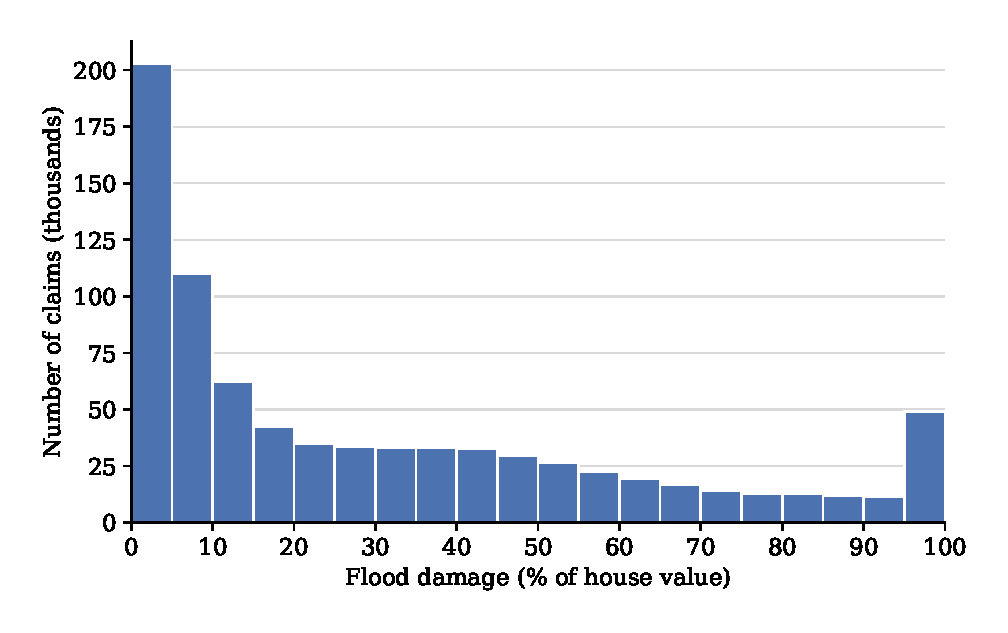
\includegraphics[height=7cm]{figures/damage_distribution.eps}
\caption{\textbf{NFIP flood damage claims since 2000.} Observations are clipped at 100$\%$ to reduce the influence of outliers and data errors.}
\label{fig:damageclaims}
\end{figure}

The ratio of income to home value behind this interpretation cannot be measured in the claims data, which contain no information on homeowners' finances. We therefore rely on aggregate statistics and use a ratio of house value to income of approximately 4, reflecting the U.S. average.\footnote{\cite{kaplan2020housing} report a skewed distribution around the turn of the century in which the median ratio of house value to income is 2.1 but the 90th percentile value is 5.5; the Harvard University JCHS reports an national ratio of 4.7 of the housing stock value over income for 2025, but this includes renters, who earn about half as much as homeowners on average (accessed via https://www.jchs.harvard.edu/sites/default/files/interactive-item/files/Harvard\_JCHS\_State\_Nations\_Housing\_2026\_Appendix\_Tables\_1.xlsx).}

% TODO (population = SFHA homeowners, decided 2026-11-07): recompute p as NFIP claims per policy-year in A/V zones only, using the same claim filter and years as the damage distribution (run_flood_arrival_rate.py currently counts all claims and reports zones separately).
Since coastal housing tends to be more expensive than inland housing, the ratio of house value to income could be different in flood-exposed areas. A simple consistency check goes as follows. From the survey evidence of \cite{qin2026flood}, for homeowners in floodplains the average NFIP insurance premium as a share of income was about 1.3$\%$ in the years 2000-2020 (ibid p. 43). Comparing claims with outstanding policies in the NFIP data, the annual arrival rate $p$ of flooding in floodplains is 1.9$\%$. Since $\overline{P}=(1-s)p\overline{d}$ and, prior to 2021, we estimate $s=0.22$ (see below), it follows that, conditional on flooding, the average ratio of expected flood damages to income is roughly 88$\%$. Relative to the average damage of about 30$\%$ of the building value, this implies a ratio of building value to income of about 2.9, which is consistent with a ratio of home value to income of about 4 if land accounts for roughly a quarter of home value. Assuming for tractability a constant ratio of home value to income in our sample, this supports the pass-through of about $0.25$ used above.
% TODO (utility base = home value incl. land; s = 0.22, both decided 2026-11-07): with s = 0.22 this calculation gives damage/income = 0.013/(0.78*0.019) = 0.88 and building value/income = 0.88/0.30 = 2.9, so home value/income = 2.9/(1 - land share), which equals 4 at a land share of about 0.27. Check against the FHFA land shares once the *_home variants are computed. The 1.3% premium share (Qin et al.) may or may not include fees; and p is still the unmatched 1.9%.
 
To do's
\begin{itemize}
\item Convert distribution of damages as \% of house value to wealth loss as in model. How? Using simple toy model with MPV? If so should be introduced in section 3, and made consistent with welfare formulas...
\item For flood arrival rate -- given the distribution of damages, make consistent with AAL reported in \cite{amornsiripanitch2025measuring}?
\end{itemize}

\subsubsection{Utility}

Households have CRRA utility $u(c)=c^{1-\gamma}/(1-\gamma)$ over consumption, with log utility for $\gamma=1$. We set $\gamma=1.5$ in our baseline. This lies between two sets of estimates. From wage and income elasticities of labor supply, \cite{chetty2006new} obtains a mean estimate of $\gamma\approx1$ and shows that values above 2 would require implausibly sharp reductions in labor supply following wage increases. From aggregate property insurance data, \cite{szpiro1986relative} reports estimates between 1.2 and 1.8 for the United States and between one and two for most other countries. We do not calibrate $\gamma$ from households' insurance choices. Deductible and coverage choices, including those of NFIP policyholders, imply relative risk aversion in the triple digits under expected utility \citep{sydnor2010overinsuring,collier2017risk}, a pattern better explained by the overweighting of small probabilities \citep{barseghyan2013nature}. In our model, such probability distortions are absorbed by the subjective beliefs $q$. We report results for $\gamma=1$ and $\gamma=3$ as robustness checks. The choice matters quantitatively, because the value of disaster aid relative to the insurance subsidy rests on the curvature of utility in the flood state.
% NB (discrete model, current calibration with s = 0.22, 2026-11-07): MVPF_a > MVPF_s at every gamma (1.15 vs 1.03 at gamma = 1). With a fixed budget, all spending goes to aid at every gamma. With fixed lambda, optimal aid rises with gamma: a* = 0.00 / 0.14 / 0.32 / 0.53 at gamma = 1 / 1.5 / 2 / 3 for lambda = 1.2, and 0.29 / 0.50 / 0.62 / 0.75 for lambda = 1.1 (s* = 0 throughout). Numbers to be reported once the calibration is final.

\subsubsection{Current policy \texorpdfstring{$(s,a)$}{(s,a)}}

In our model, $s$ is the wedge between the flood insurance premium paid by the household and its expected insurance pay-out. It is not (minus) the balance of the NFIP divided by its revenues, which also reflects administrative costs. Since part of these costs is financed through loads in the premium, measuring $s$ against expected claims rather than against the full-risk premium matters for its value (see below). Administrative costs are an important consideration in practice, and we discuss them in section \ref{subsec:admincosts}.

As mentioned in section \ref{subsec:insurance}, current policy is not stable, because the RR2.0 reform has set insurance premiums on a gradual path towards actuarially fair rates. Based on the availability of high-quality empirical studies, we calibrate our ``current policy MVPF'' formulas from data just \textit{before} the NFIP reform; accordingly, the value of $s$ is positive.

There is a range of estimates reported in the literature for the NFIP subsidy rate, some ex-ante (comparing premiums to estimated flood risk) and some ex-post (comparing premiums to realized flood events). The ex-post estimate of \cite{wagner2022adaptation} is a subsidy of 30\%. Ex-ante estimates compare premiums before RR2.0 with the full-risk premiums that FEMA is now phasing in. \cite{gruber2026optimal} find that average premiums rise from $\$$944 to $\$$1,739, which implies a subsidy of 46\%, and \cite{bakkensen2020sorting} obtain about 50\% in a sample of Florida properties, reflecting pre-FIRM and CRS discounts built into the system prior to RR2.0. However, full-risk premiums exceed expected claims. Besides the average annual losses from catastrophe models, they include provisions for the expense allowance of the private insurers that sell NFIP policies, about 30\% of the premium, as well as for loss adjustment expenses, reinsurance and a load for catastrophic risk \citep{gao2023flood}. Netting out the expense allowance alone gives a subsidy relative to expected claims of $1-944/(0.7\cdot1{,}739)\approx0.22$. This is an upper bound, since we cannot net out the other provisions. In addition, policyholders pay assessments, surcharges and fees on top of the premium \citep{gao2023flood}; counting these, the pre-reform subsidy relative to expected claims is close to zero. We set $s=0.22$ in our baseline and report results for $s=0$ and $s=0.46$ as robustness checks.

For the disaster aid fraction $a$, which in our model is both the household's benefit and the government's cost per dollar of uninsured damage, we only count transfers paid directly to households: IHP grants, and SBA loans at their subsidy-equivalent value of 13 cents per dollar lent \citep{gruber2026optimal}. These amount to about $\$$1.75bn per year: $\$$1.55bn of IHP grants over 2003--2024 \citep{crs2025ihpfaq}, and $\$$0.20bn for SBA home loans, which averaged $\$$1.57bn per year over 2003--2022 \citep{sba2022disaster}. Of this, we attribute 48.9$\%$ to flooding based on OpenFEMA disaster summaries. Dividing by uninsured residential flood damage, 82$\%$ of about $\$$20bn per year \citep{firststreet2021cost},\footnote{This is the modeled expected annual loss for 1--4 unit residential homes with substantial flood risk. Using the same flood model, \cite{wing2022inequitable} estimate average annual losses of $\$$32.1bn for all property types, including commercial buildings.} gives $a\approx0.052$. Although these figures are national, we apply the resulting rate to homeowners in SFHAs, which assumes that aid per dollar of uninsured damage does not differ systematically between SFHAs and other flood-prone areas.

We do not adopt the IV estimate of $a=0.133$ by \cite{gruber2026optimal}, as it measures how total federal outlays respond to insurance coverage rather than the transfer per dollar of damage. It thereby includes mitigation grants (HMGP), mortgage losses, and indirect channels such as interactions with NFIP payouts. Indeed, their own average aid payments per flood-affected house imply an $a$ of only 0.031--0.036. Our estimate is uncertain mainly because of the flood share of IHP spending, which lies between 9.3$\%$ (disasters declared as floods) and 88.6$\%$ (including hurricanes and storms) and implies a range for $a$ of 0.010--0.095. We use the estimate of \cite{gruber2026optimal} restricted to IHP and SBA, $a=0.12$, as an upper bound in our robustness checks.

\subsubsection{Insurance take-up}
Although 59.5\% of homeowners within SFHAs hold some flood insurance, only 48.4\% of expected flood damages are insured as not all homeowners purchase full insurance (see \cite{amornsiripanitch2025measuring}; statistics as of 2023). In our model with a binary insurance decision, the aggregate insurance rate equals the percentage of expected damages covered. We therefore set $I=0.484$, including both voluntary and mandated insurance demand. 

Only households that are not subject to the insurance mandate respond to policy. The share $\phi$ of mandated households therefore matters only for the optimal policy, and we calibrate it in Section~\ref{subsec:calib_phi}.    

Several estimates exist in the literature for the price elasticity of flood insurance demand. \cite{mulder2024mismeasuring} exploits NFIP map adjustments transferring homeowners into high-risk SFHAs, which are accompanied by price increases at different calendar dates. He arrives at a price elasticity of insurance demand of $-0.177$ (and $-0.37$ for voluntary demand). \cite{wagner2022adaptation}, using price variation from the Biggert-Waters and HFIAA reforms of the NFIP, obtains a price elasticity of $-0.25$ in SFHAs. Finally, \cite{gruber2026optimal} estimate the response of policy renewals to the capped premium increases after the RR2.0 reform, obtaining an elasticity of $-0.32$ across all flood zones and $-0.25$ within SFHAs. Since our population consists of homeowners in SFHAs, we set $\epsilon=-0.25$ in our baseline, on which two independent research designs within SFHAs agree. We use the estimates of $-0.177$ and $-0.32$ as lower and upper bounds in our robustness checks.         

Inserting our estimates for the elasticity, $I$ and $s$ into \eqref{eq:insurancedemandwrts} gives $\partial I/\partial s=0.16$. It should be emphasized again that this is a local estimate that holds given current policy $(s,a)$; the response of take-up to disaster aid follows from \eqref{eq:insurancedemandwrta}.

\subsection{Optimal policy}\label{subsec:calib_optimal}

The current-policy MVPFs depend on the distribution of beliefs only through the density at the margin, which we recover from the observed premium elasticity. To solve for the optimal policy $(s^*,a^*)$, we need three further objects: the share $\phi$ of households subject to the insurance mandate, the full belief distribution $F(q)$ of the remaining households, and the budget available to the planner.

\subsubsection{Mandated share}\label{subsec:calib_phi}

Regarding the fraction $\phi$, \cite{mulder2024mismeasuring} finds in his survey of homeowners in high-risk areas that 39\% are subject to a mandatory insurance requirement. He uses that number to convert an estimate for the price elasticity of insurance demand to an estimate for \textit{voluntary} insurance demand. For our purposes, an important adjustment comes from the fact that the purchase requirement is partial.\footnote{It is capped at the minimum of the value of the mortgage, the NFIP coverage limit of $\$250,000$, and the replacement value of the property.} Unfortunately, there is no data to compare the intensive margin of the insurance decision between homeowners with and without a mortgage.\footnote{Researchers have been unable to match individual-level mortgage data with publicly available NFIP policies and claims data because the latter are anonymized; \cite{mulder2024mismeasuring}'s survey avoids this problem.} We therefore assume their policies on average cover the same fraction of expected damages and set $\phi=0.39\cdot\frac{0.484}{0.595}=0.32$.\footnote{Our model treats the mandate as independent of beliefs, but mandated households appear to perceive higher risk. Of homeowners subject to the requirement, 53$\%$ report that they would be extremely likely to buy flood insurance without it \citep[p.~16]{mulder2024mismeasuring}, and these households report a roughly 50$\%$ higher willingness to pay than voluntary buyers (ibid., Appendix D). This does not affect our calibration, since the belief distribution is identified only from the decisions of households not subject to the mandate. It does imply that the beliefs we recover are likely lower than those of the average homeowner in surveys that include mandated households.} It follows that the \textit{voluntary} insurance take-up rate inside SFHAs is approximately 24.5\%, which is significantly higher than the rate of 16.3\% outside SFHAs.\footnote{See \cite{amornsiripanitch2025measuring}, p. 969: in flood-prone areas outside SFHAs, 22\% of households hold a policy and 16.3\% of expected damages are covered.}

\subsubsection{Belief distribution}

We assume that the beliefs of households not subject to the mandate follow a Beta distribution with parameters $(\alpha,\beta)$, a flexible two-parameter family on the unit interval. The two parameters are exactly identified by two moments at current policy: voluntary take-up, $1-F(q^*)=(I-\phi)/(1-\phi)$, and the density at the margin $f(q^*)$ implied by the premium elasticity, eq.~\eqref{eq:fqstar}. By construction, the fitted distribution reproduces the observed take-up and its response to policy, so that the optimal-policy MVPFs~\eqref{eq:mvpf_deep_prog} coincide with the current-policy MVPFs~\eqref{eq:mvpf_prog} at current policy.

We do not use survey data on flood risk beliefs in the calibration, but use them to validate the fitted distribution. Two surveys provide benchmarks. \cite{bakkensen2022going} elicit flood risk beliefs of coastal homeowners in Rhode Island. They find a mean belief of 57\% of the objective risk, and 35\% of respondents perceive a 10-year flood probability of at most 5\%. In the survey of \cite{mulder2024mismeasuring}, homeowners inside the floodplain report a mean 10-year flood probability of 27.75\% (ibid., Table A1), or about 3\% per year, above the objective rate in our calibration. The two benchmarks thus differ by a factor of about three. Both include households subject to the mandate, who perceive higher risk (Section~\ref{subsec:calib_phi}), and stated probabilities of rare events tend to be overweighted.

The fitted distribution has a shape parameter $\alpha$ below one, so that its density is highest at very low beliefs. Its mean belief is [TO DO: value] of the objective risk, and [TO DO: value] of households have a 10-year belief of at most 5\%, compared with 35\% in the survey of \cite{bakkensen2022going}. The fitted distribution thus places more households at very low beliefs than the survey evidence suggests. We interpret the fitted $q$ as decision weights, which absorb probability distortions and other frictions in insurance decisions, rather than as literal beliefs. Section~\ref{subsec:functionalform} reports results for alternative functional forms, including a mixture with a mass of households who never insure.
% Values (2026-11-08; s = 0.22, a = 0.052, gamma = 1.5, building-value base, no loss cap):
%   mean-damage model: Beta(0.313, 26.1), q* = 0.74p, mean 0.59p, 58% with 10-year belief <= 5%.
%   empirical damages (FEMA, uncapped): Beta(0.314, 66.3), q* = 0.29p, mean 0.24p, 74%.
%   Report once the tail treatment (loss cap) and the home-value base are final (notes/calibration_overview.md 3.3-3.5).

\subsubsection{Budget}

In the planner problem of Section~\ref{sec:model}, the planner allocates a budget $B$ between the two instruments, eq.~\eqref{eq:budget_prog}. We set the budget equal to current spending, $B_0=p\overline{d}\,[sI+a(1-I)]$ evaluated at current policy, of which about 20\% is spent on disaster aid. The optimal policy then answers how a given amount of public spending on flood policy should be divided between the insurance subsidy and disaster aid, and $\lambda$ is the multiplier on this budget. As a secondary exercise, we instead fix the marginal cost of public funds and let total spending adjust, using $\lambda=1.2$, the value used by \cite{gruber2026optimal} in their robustness checks, and $\lambda=1.1$.

Table~\ref{tab:calibration} summarizes the baseline calibration. The parameters in all but the last group are all that the current-policy MVPFs require; in particular, they do not require the belief distribution $F(q)$, since the density at the margin $f(q^*)$ is recovered from take-up and its premium elasticity (Section~\ref{subsec:fqstar}). The last group enters only the optimal policy.

\begin{table}[htbp]
\centering
\caption{\textbf{Baseline calibration (homeowners in SFHAs).}}
\label{tab:calibration}
\footnotesize
\renewcommand{\arraystretch}{1.2}
\begin{tabularx}{\textwidth}{@{}>{\raggedright\arraybackslash}p{3.1cm} >{\centering\arraybackslash}p{1.5cm} >{\centering\arraybackslash}p{1.6cm} >{\raggedright\arraybackslash}X >{\raggedright\arraybackslash}p{3.7cm}@{}}
\toprule
Parameter & Baseline & Robustness & Target / interpretation & Source \\
\midrule
\multicolumn{5}{@{}l}{\textit{Flooding process}} \\
Flood probability $p$ & 0.019 & & NFIP claims per policy in force in floodplains & NFIP claims and policies \\
Damages $G(d)$ & empirical & excl.\ Katrina & Claimed damage relative to home value incl.\ land (mean 30\% of building value) & NFIP claims; \cite{davis2019land} \\
\cmidrule[0.2pt]{1-5}
\multicolumn{5}{@{}l}{\textit{Utility}} \\
Risk aversion $\gamma$ & 1.5 & 1, 3 & Between labor-supply and property-insurance estimates & \cite{chetty2006new}; \cite{szpiro1986relative} \\
Resources $w$ & home value & & Pass-through of losses to consumption $\approx$ income/home value $\approx 0.25$ & \cite{kaplan2020housing}; \cite{davis2019land} \\
\cmidrule[0.2pt]{1-5}
\multicolumn{5}{@{}l}{\textit{Current policy}} \\
Premium subsidy $s$ & 0.22 & 0, 0.46 & Premium paid relative to expected claims, before RR2.0 & \cite{gruber2026optimal}; \cite{gao2023flood} \\
Disaster aid $a$ & 0.052 & 0.12 & IHP grants and SBA loan subsidies for floods, per dollar of uninsured residential damage (range 0.010--0.095) & \cite{crs2025ihpfaq}; \cite{sba2022disaster}; \cite{firststreet2021cost}; \cite{gruber2026optimal} \\
\cmidrule[0.2pt]{1-5}
\multicolumn{5}{@{}l}{\textit{Insurance take-up}} \\
Take-up $I$ & 0.484 & & Share of expected flood damages insured in SFHAs (2023) & \cite{amornsiripanitch2025measuring} \\
Premium elasticity $\epsilon$ & $-0.25$ & $-0.177$, \newline $-0.32$ & Elasticity of total take-up in SFHAs & \cite{wagner2022adaptation}; \cite{gruber2026optimal}; \cite{mulder2024mismeasuring} \\
\cmidrule[0.2pt]{1-5}
\multicolumn{5}{@{}l}{\textit{Implied}} \\
$\partial I/\partial s$ & 0.16 & & $-\epsilon I/(1-s)$, eq.~\eqref{eq:insurancedemandwrts} & \\
\cmidrule[0.2pt]{1-5}
\multicolumn{5}{@{}l}{\textit{Optimal policy only}} \\
Mandated share $\phi$ & 0.32 & & Share subject to the purchase requirement (39\%), scaled by average coverage & \cite{mulder2024mismeasuring} \\
Beliefs $F(q)$ & Beta & other forms & Fitted to voluntary take-up and the density at the margin $f(q^*)$; validated against surveys & \cite{bakkensen2022going}; \cite{mulder2024mismeasuring} \\
Budget $B$ & current spending & fixed $\lambda$: 1.1, 1.2 & Spending on subsidy and aid at current policy (20\% on aid) & eq.~\eqref{eq:budget_prog}; \cite{gruber2026optimal} \\
\bottomrule
\end{tabularx}

\vspace{0.5ex}
\begin{minipage}{\textwidth}\footnotesize
\textit{Notes:} Robustness values are reported in Section~\ref{sec:robustness}. The parameters in the last group enter only the optimal policy (Section~\ref{subsec:calib_optimal}); the mandated share $\phi$ cancels out of the current-policy MVPFs.
\end{minipage}
\end{table}
% NB: the code uses p = 0.02 (params.P); p and the mean damage relative to home value are to be updated (see TODOs in the flooding-process subsection).

\section{Results}
\label{sec:results}

\section{Robustness}
\label{sec:robustness}
\subsection{Redistributive effects}
Households vary in their wealth and income, which bears on their exposure to flooding and their demand for flood insurance. Thus, the insurance premium subsidy and disaster aid may  have redistributive effects.

\cite{qin2026flood} combine comprehensive census and property tax records for the whole of the United States to document a number of facts. First, moving across the income distribution, the fraction of households living in a floodplain is essentially flat, hovering between around 13$\%$ in the left tail to just under 12$\%$ around the 75th percentile, with however a spike in the top income decile reaching around 18$\%$ (ibid p. 31). Second, relative to income, both homeowners' insurance premiums and their expected losses from flooding fall considerably with income, and with a comparable slope (ibid p. 44 and p. 46). Third, the insurance rate rises with income -- moving from the 25th to the 75th income percentile, the fraction of uninsured households in floodplains falls by about half (ibid p. 45).\footnote{Compared to the administrative NFIP data of \cite{amornsiripanitch2025measuring}, the survey data of \cite{qin2026flood} indicate a higher insurance rate overall.} 

Both the insurance subsidy and disaster aid do little for the poorest households which do not own housing. Within the group of homeowners, the fact that the flood insurance rate and the value of insured housing rises with income would make the insurance subsidy regressive. Regarding disaster aid, eligibility for SBA loans is tied to homeowners' credit score and income and so skewed towards higher-income households. Furthermore, although eligibility for IHP grants should be independent of victims' identity, \cite{billings2022let} uncover that households in lower-income neighborhoods receive less funds conditional on damages. Overall, then, both instruments may be regarded as somewhat regressive in their design and even more so in their effect.

To the extent that redistributive concerns affect the marginal value of either instrument, the optimal level of both the insurance subsidy and disaster aid is reduced. We note, however, that while redistribution should be aimed at lifetime earnings, both policy instruments exist to reduce the immediate drop in consumption (and rise in bankruptcies) that follows from households' limited ability to obtain credit in the aftermath of a flood.  

\subsection{Demand for adapted housing}

\subsection{Administrative costs}\label{subsec:admincosts}

Here, enter some available estimates. 

\subsection{Functional form belief distribution}\label{subsec:functionalform}

\subsection{Dispersion in risk aversion}
\section{Conclusion}
\label{sec:conclusion}

\bibliographystyle{apacite}
\bibliography{bibfile.bib}
\end{document}